\documentclass[border=0.2cm]{standalone}
\usepackage{tikz}
\usetikzlibrary{calc}
\begin{document}


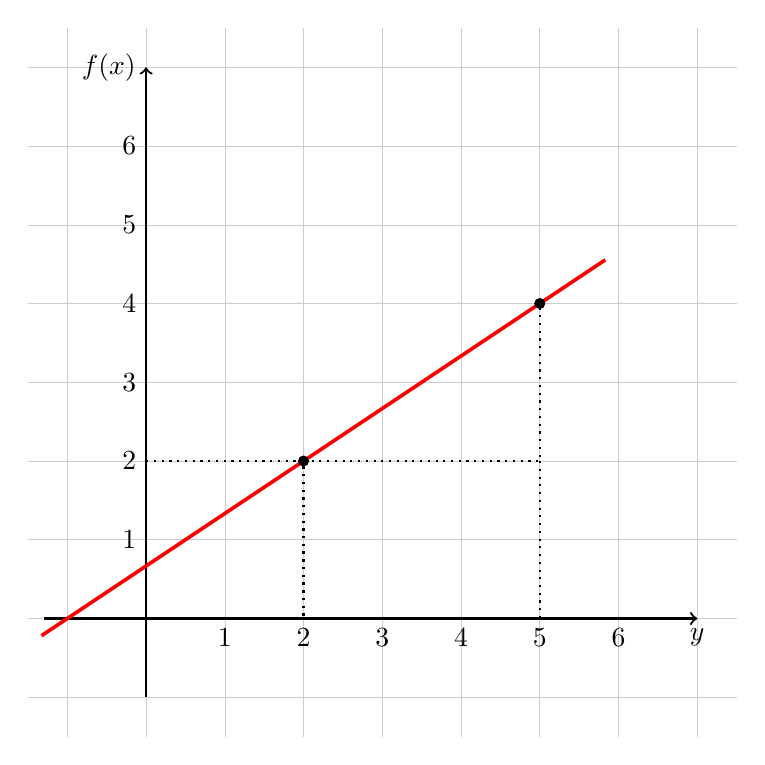
\begin{tikzpicture}
  \coordinate (a) at (0,0); 
  \coordinate (b) at (2,2);
  \coordinate (c) at (5,4);
  \draw[help lines,black!20] (-1.5,-1.5) grid (7.5,7.5);
  \foreach \x in {1,...,6} \node[left] at (0,\x) {\x} node[below] at (\x,0) {\x};
  \draw[thick,->] (0,-1) -- (0,7) node[left] {$f(x)$};
  \draw[thick,->] (-1.3,0) -- (7,0) node[below] {$y$};
  \draw[line width=1.3pt,red] ($(b)!-4cm!(c)$) -- ($(c)!-1cm!(b)$);
  \draw[thick, dotted] (0,2) -- (b) -- (2,0) -- (b) -- (5,2) -- (5,4);
  \draw[thick, dotted] (5,2) -- (5,0);
  
%  \fill[color=black] (a) circle (2pt);% node[right] {(a)};
  \fill[color=black] (b) circle (2pt);% node[right] {(b)};
  \fill[color=black] (c) circle (2pt);% node[right] {(c)};

  %\draw (-2,0) circle (1pt) node[left] {$f(x_1)$};
  %\draw (-2,1) circle (1pt) node[left] {$f(x_2)$};
%  %\draw[thick, dotted] (-2,1) -- +(3,0) -- (1,-1) node[below] {$x_2$};
%  %\draw[thick, dotted] (0,0) -- (1,0);
%  %\draw[thick] (.5,0) arc (0:45:0.5) node[right] {$\alpha$};
%  %\fill (1,1) circle (1.2pt);
%  %\fill (0,0) circle (1.2pt);
\end{tikzpicture}



\end{document}